Adesso teniamo conto delle perturbazioni che l'orbita del satellite subisce,
andando quindi a calcolare la risposta forzata, considerando la non sfericità
della Terra e la presenza delle forze non gravitazionali. Vi sono diversi tipi
di orbite che possono essere realizzate, nel nostro caso l'orbita sarà
elio-sincrona, quindi i raggi solari andranno a colpire sempre la stessa faccia
del satellite. Poiché la direzione Sole-Terra ruota per tutta la durata
dell'anno solare, il piano orbitale non può rimanere fisso nello spazio, ma la
linea dei nodi deve ruotare, introducendo così il moto di precessione. Per fare
ciò bisogna far ruotare l'asse dei nodi per mantenere il piano orbitale sempre
con lo stesso angolo ripetto la direzione Sole-Terra
\begin{equation}
\omega_s\approx \frac{2\pi}{365.25\times86400}\approx 0.2 \ \mu rad/s
\end{equation}
Un'orbita di questo tipo è non kepleriana, ma possiamo sfruttare le
perturbazioni esterne per assicurarci il moto di precessione. Si può dimostrare
che grazie alll'appiattimento terrestre, ad una specifica inclinazione del piano
orbitale, dipendente dall'eccentricità e dalla lunghezza del semi-asse maggiore,
il moto di precessione viene perseguito in maniera naturale. Considerando il
nostro caso, ovvero un'orbita ad una bassa altitudine e una piccola eccentricità
e considerando la costante $J_2$, per assicurarci il
moto di precessione l'orbita dev'essere di tipo quasi-polare.
Come accennato in precedenza è necessario tenere conto di ogni causa che può
modificare l’orbita del satellite. I principali fattori di cui tenere conto
sono: le anomalie del campo gravitazionale, le forze elettromagnetiche, e le
forze aerodinamche o di attrito. Focalizzeremo l'attenzione sulle forze
di attrito (drag forces), ovvero le perturbazioni causate dalle molecole
dell'atmosfera rarefatta. Azzerare queste perturbazioni è lo scopo del controllo
drag-free.
In base alle proprietà della superficie del satellite, inclusa la sua
temperatura, le molecole dell'atmosfera incidono su di essa in due differenti
modi, figura \ref{fig:riflessione}
\begin{itemize}
  \item Riflessione speculare (o elastica), avviene quando le molecole
  rimbalzano sulla superficie senza perdita di energia, ciò implica che la
  velocità di uscita delle molecole $\vec{v_0}$ è complanare alla velocità
  $\vec{-v_r}$ con la quale impattano la superficie e gli angoli di incidenza e
  di riflessione sono uguali
\begin{equation}
\begin{array}{l}
\vec{v_r}=v_r(\cos{\alpha \vec{n}}-\sin{\alpha \vec{t}}) \\
\Delta \vec{v_s}=((\vec{-v_r}\vec{-v_r})\vec{n})\vec{n} +
((\vec{-v_r}\vec{+v_r})\vec{t})\vec{t} = -2v_r\cos{\alpha \vec{n}}
\end{array}
\label{eq:specular}
\end{equation}
  \item Riflessione diffusa (o termica), si ha quando le particelle che
  colpiscono la superficie perdono tutta la loro energia nell'impatto.
  L'assorbimento delle molecole dipende dalla temperatura della superficie del
  satellite
\begin{equation}
\begin{array}{l}
\vec{v_d}=v_d(\theta_s)\vec{n} \\
\Delta\vec{v_d}=((\vec{-v_d}\vec{-v_r})\vec{n})\vec{n} +
((\vec{-v_d}\vec{-v_r})\vec{t})\vec{t}
= -(v_r\cos{\alpha}+v_d)\vec{n}-v_r\sin{\alpha}\vec{t}
\end{array}
\label{eq:diffusion}
\end{equation}
\end{itemize}

\begin{figure}[htp]
\begin{center}
  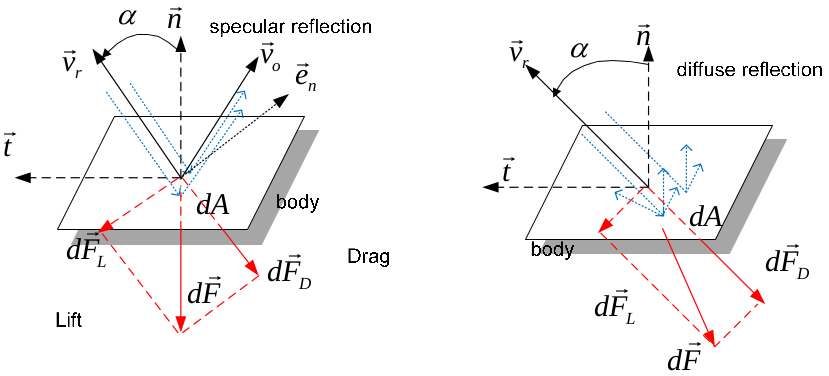
\includegraphics[width=\textwidth]{modelling/orbit_dynamics/image/riflessione.png}
  \caption{Riflessione speculare e diffusa su di una superficie}
  \label{fig:riflessione}
\end{center}
\end{figure}

Il momento totale per unità di massa lo si ottiene combinando le due equazioni
\ref{eq:specular} e \ref{eq:diffusion} e considerando due coefficienti
$0\leq\sigma_t$ e $\sigma_n\leq 1$ che pesano le componenti tangenziale e
normale di incisione
\begin{enumerate}
  \item $\sigma_t = \sigma_n = 0$, riflessione speculare
  \item $\sigma_t = \sigma_n = 1$, riflessione diffusa
\end{enumerate}
Il momento totale risutla essere
\begin{equation}
\Delta\vec{v} = ((2 - \sigma_n)v_r\cos{\alpha} + \sigma_nv_d)\vec{n}+\sigma_t
v_r \sin{\alpha\vec{t}}
\end{equation}
Moltiplicando il flusso della massa atmosferica $d\phi$ sulla superficie per il
momento totale, otteniamo la forza aerodinamica totale
\begin{IEEEeqnarray}{rCl}
d\vec{F}&=&d\phi\Delta \vec{v}= -\rho\vec{v_r}\cdot \vec{n}dA\Delta\vec{v}=
\nonumber \\&=& -\rho v_r^2\cos{\alpha}(((2-\sigma_n)\cos{\alpha} + \sigma_n
v_d/v_r)\vec{n} + \sigma_t \sin{\alpha}\vec{t})dA
\label{eq:aero_force}
\end{IEEEeqnarray}

In caso di pura diffusione, condizione molto simile alla realtà, e assumendo
$v_d / v_r \approx 0$, l'equazione \ref{eq:aero_force} diventa
\begin{equation}
d\vec{F}=-\rho v_r^2 \cos{\alpha} \sigma_t\vec{e}_v dA
\end{equation}
Il che dimostra che la forza aerodinamica è diretta lungo il flusso incidente la
superficie del satellite.
Scomponendo la superficie normale nel vettore velocità e nella sua
perpendicolare
\[ \vec{n}= \cos{\alpha}\vec{e}_v + \sin{\alpha}\vec{e}_n \]
La forza aerodinamica la si può scrivere come somma del componente di 'drag' e
di 'lift'
\begin{equation}
d\vec{F}=d\vec{F}_D+d\vec{F}_L=-\frac{1}{2}\rho
v_r^2(C_D\vec{e}_v+C_L\vec{e}_n)dA
\end{equation}
dove
\[
C_D=2\cos{\alpha}(\sigma_t+(2-\sigma_n-\sigma_t)\cos^2{\alpha}+\sigma_n\cos{\alpha}
\ v_d/v_r) \]
\[ C_L=2\cos{\alpha}\sin{\alpha}((2-\sigma_n-\sigma_t)\cos{\alpha} + \sigma_n \
v_d/v_r)
\]

Adesso siamo pronti ad avviare la simulazione con i seguenti parametri settati
\begin{lstlisting}[language=matlab,breaklines=true]
GravityTypeFlag=1;		%(1=J2 Gravity Model/=0 Spherical)
GravityGradientTorqueFlag=1;	%1=Gravity Gradient Torque ON/0=OFF 
DragForceDisturbancesFlag=1;	%0=Drag Force Disturbance OFF/1=OFF
DragTorquesDisturbancesFlag=1;	%0=Drag Torque Disturbance OFF/1=ON
DragFreeControlFlag=0;		%0=Drag Free Control OFF/1=ON
AttitudeControlFlag=0;		%0=Attitude Control OFF/1=ON
\end{lstlisting}


Per quanto concerne la visualizzazione dei plot della simulazione, sono
rappresentati i sei parametri orbitali, sia in caso di risposta libera, che in
caso di risposta forzata.

\begin{SCfigure}[0.7][ht]
	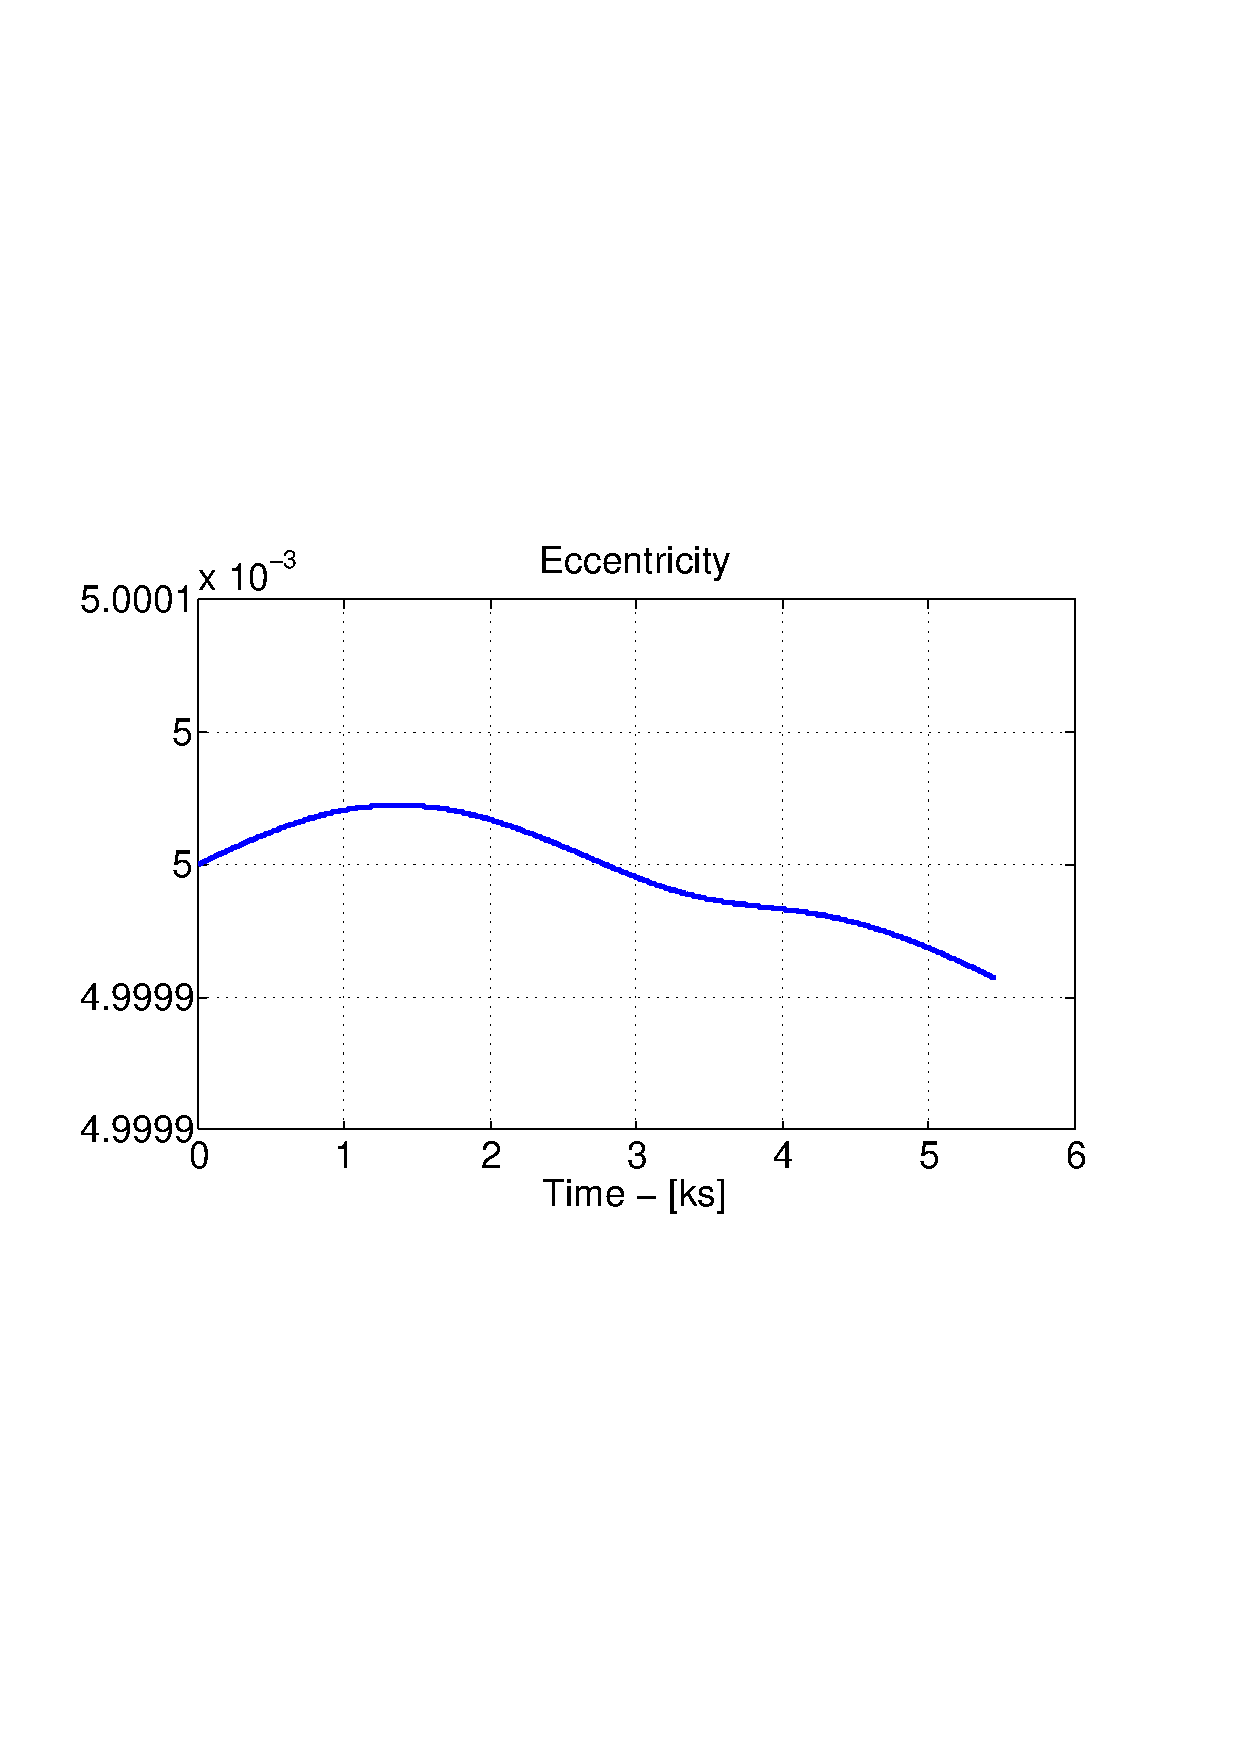
\includegraphics[width=.6\textwidth,clip=true,trim=1cm
	6cm
	1cm
	8cm]{modelling/orbit_dynamics/image/eccentricity.pdf}
	\caption{\emph{Eccentricità}}
\end{SCfigure}

\begin{SCfigure}[0.7][ht]
	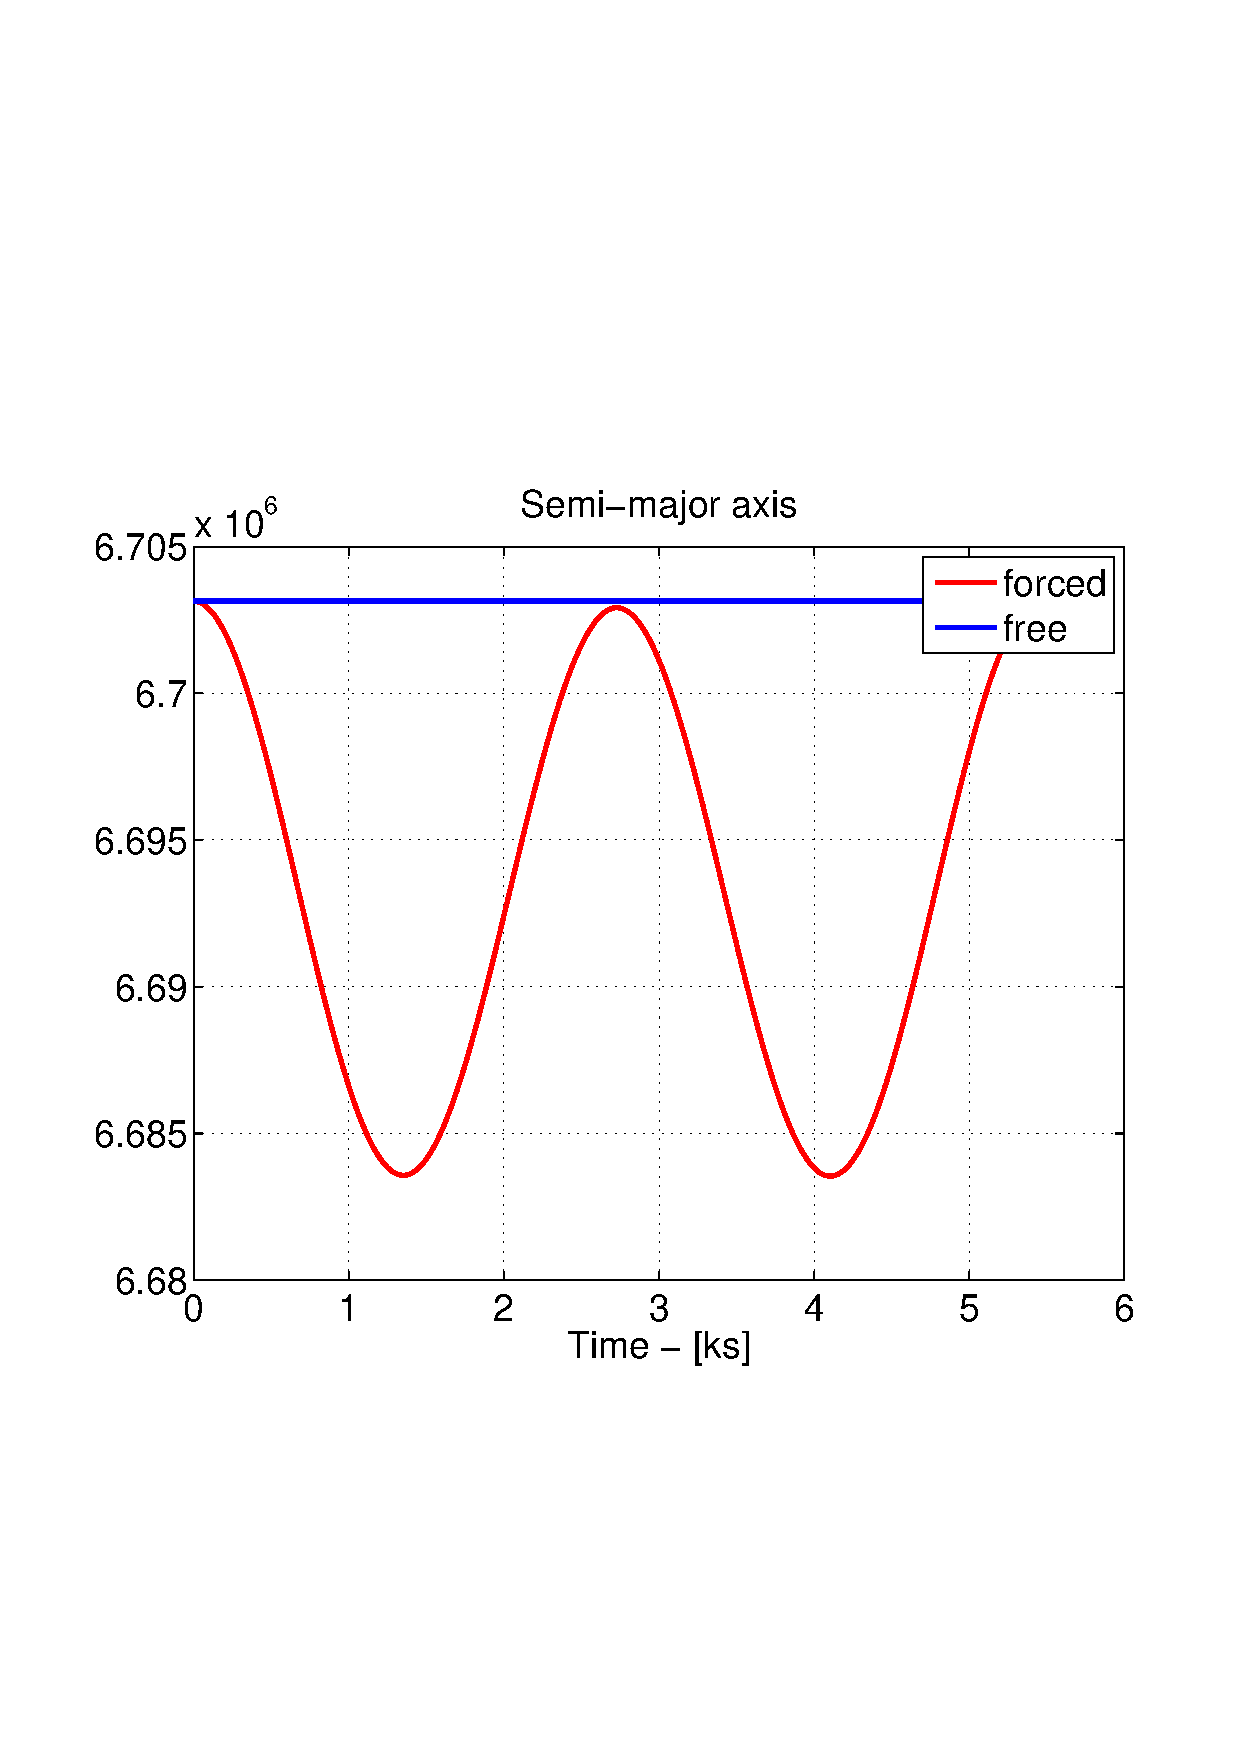
\includegraphics[width=.6\textwidth,clip=true,trim=1cm
	6cm
	1cm
	8cm]{modelling/orbit_dynamics/image/semi-major_axis.pdf}
	\caption{\emph{Semi-asse maggiore}}
\end{SCfigure}

\begin{SCfigure}[0.7][ht]
	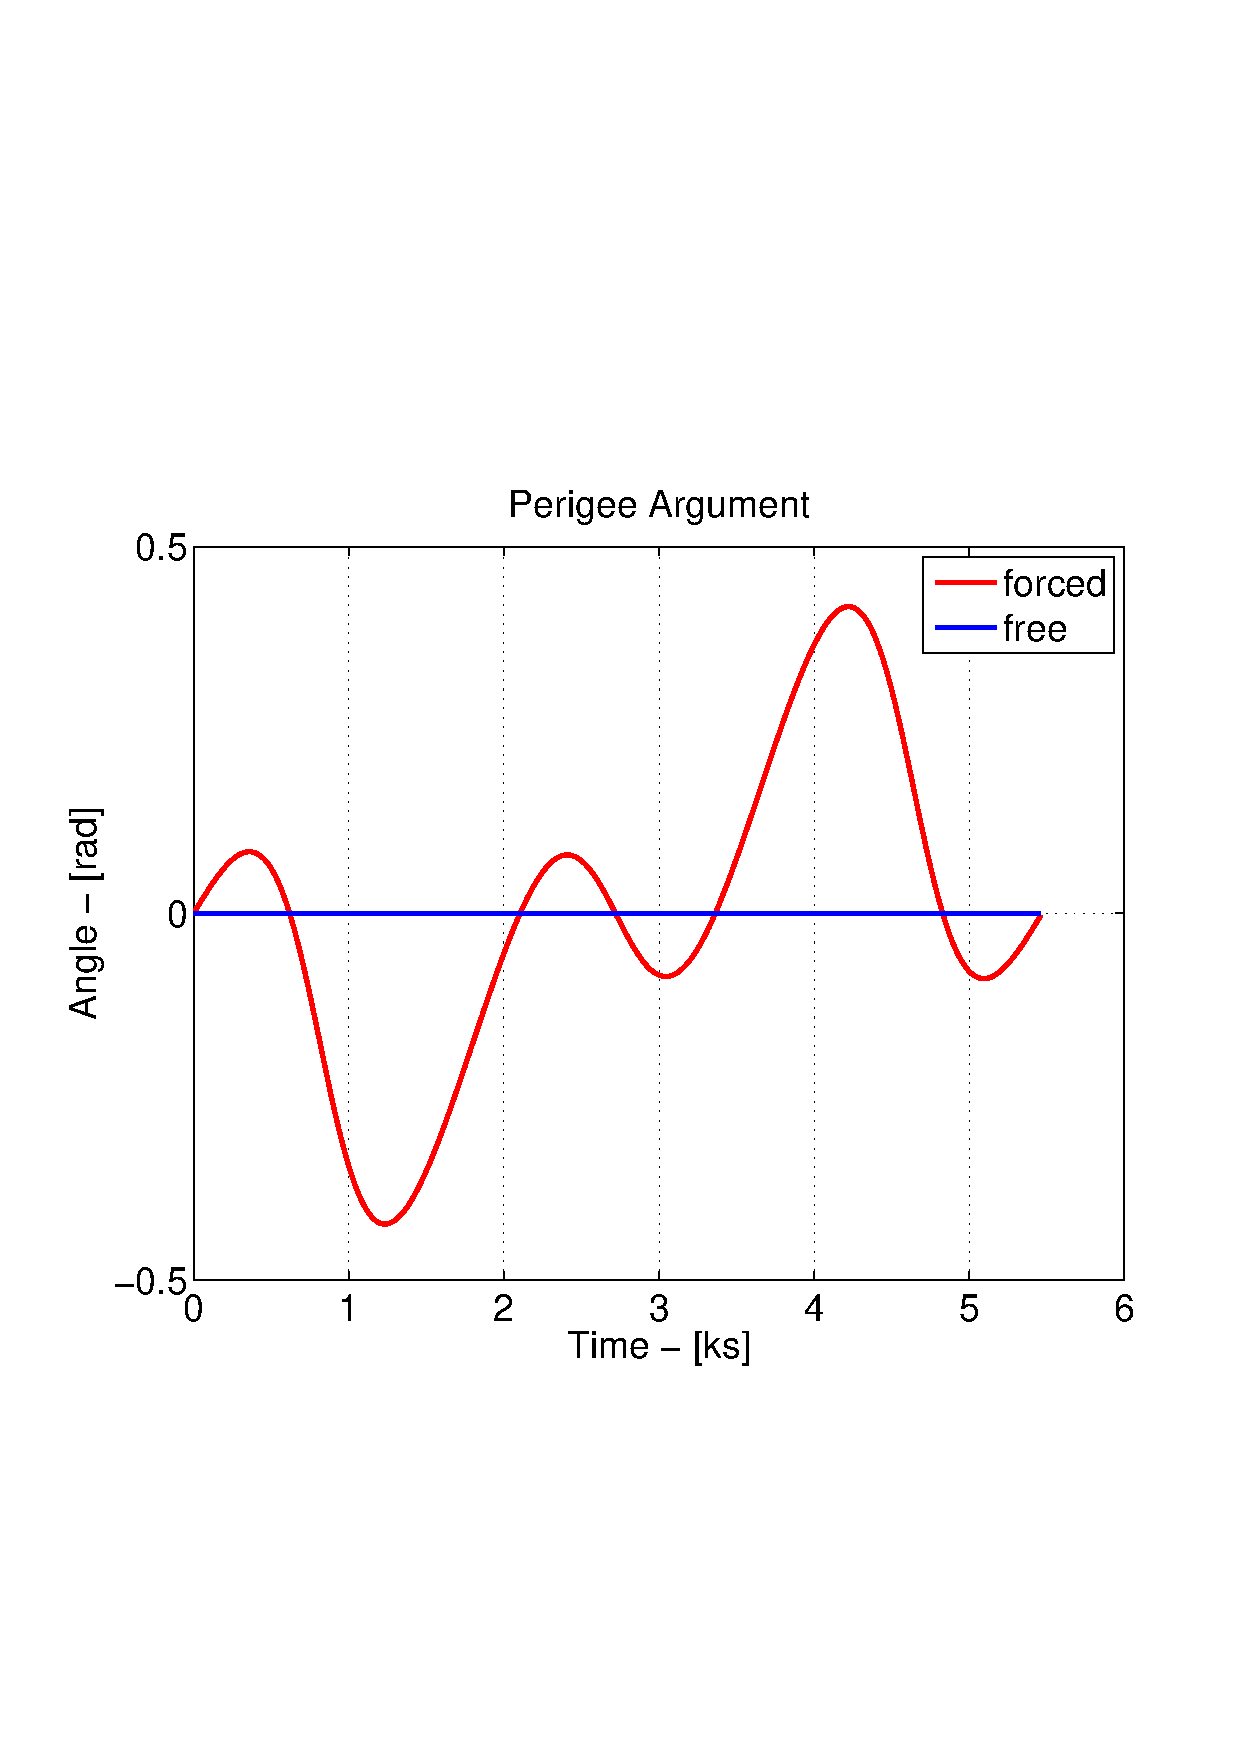
\includegraphics[width=.6\textwidth,clip=true,trim=1cm
	6cm
	1cm
	8cm]{modelling/orbit_dynamics/image/perigee_argument.pdf}
	\caption{\emph{Argomento del perigeo}}
\end{SCfigure}

\begin{SCfigure}[0.7][ht]
	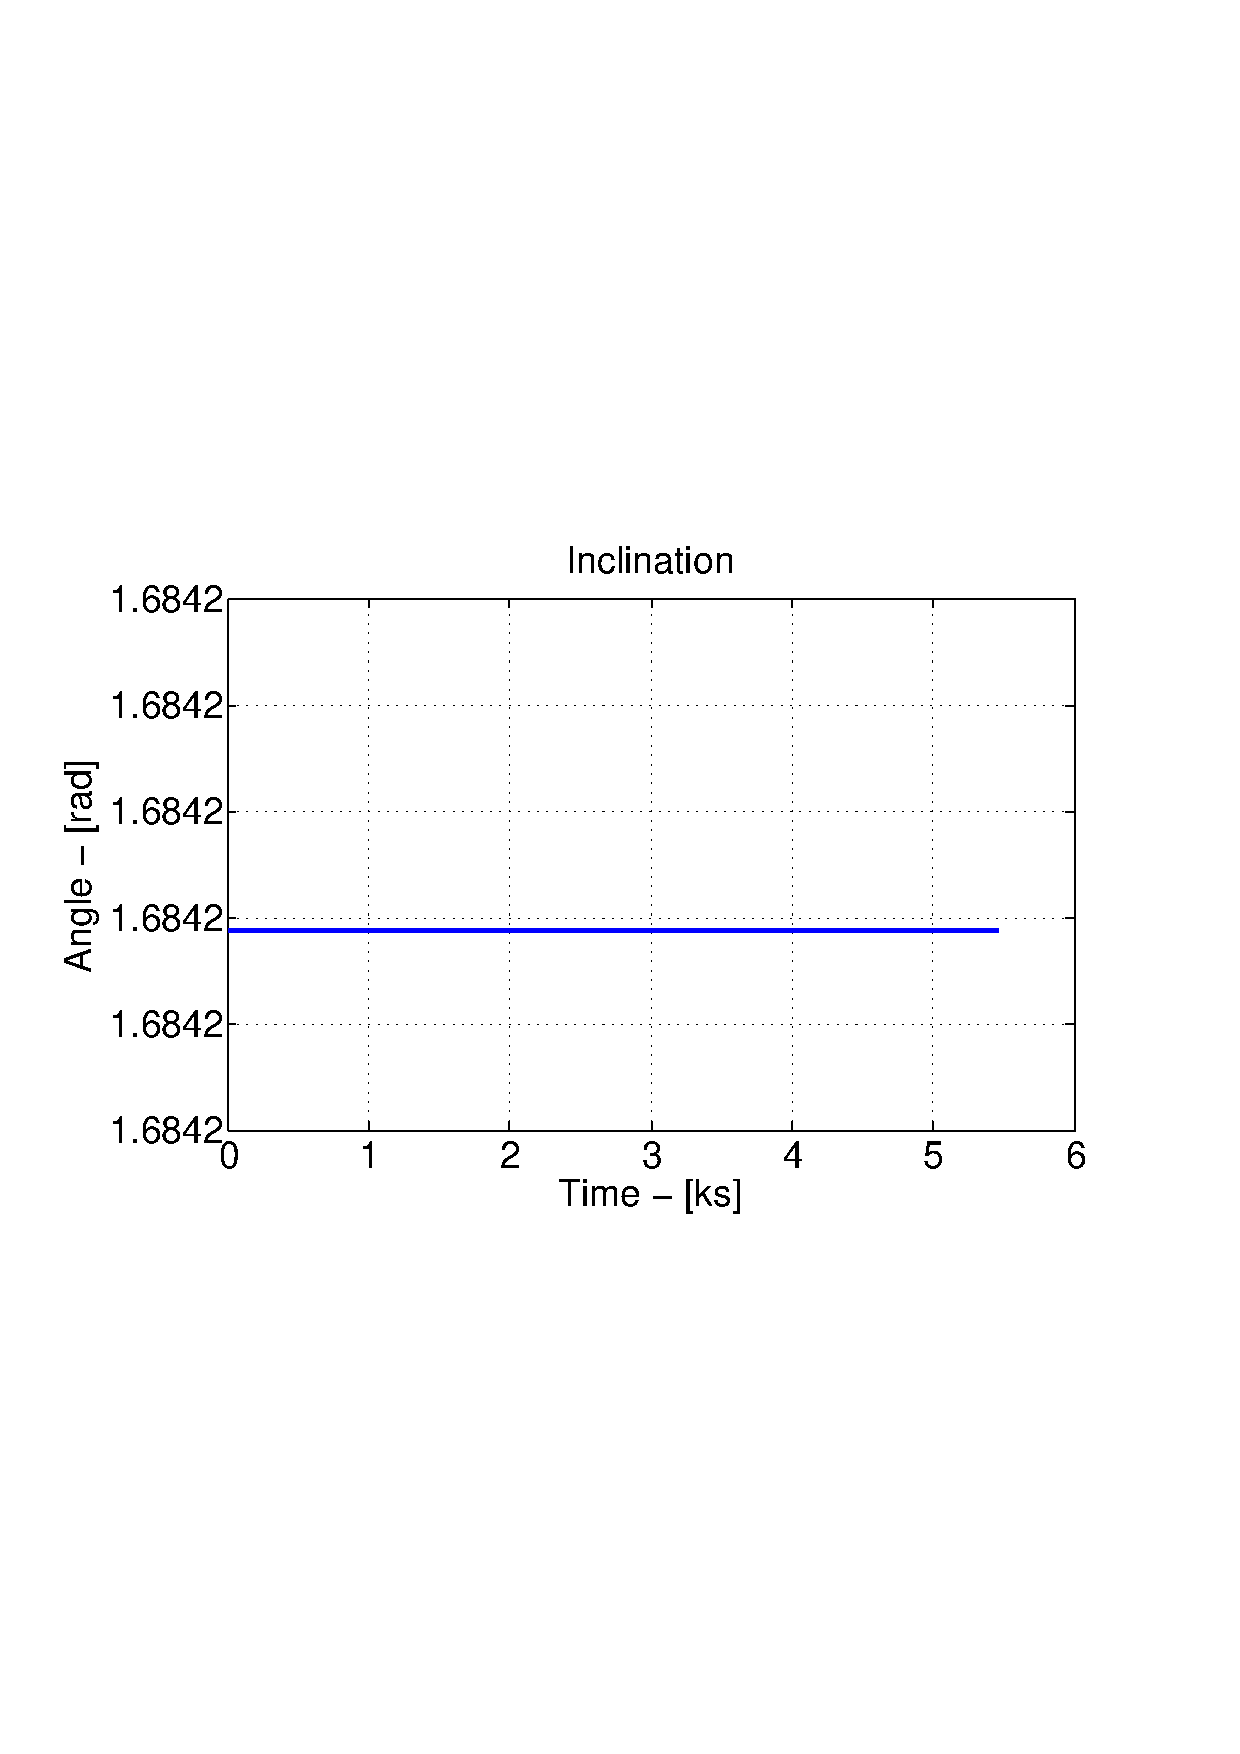
\includegraphics[width=.6\textwidth,clip=true,trim=1cm
	6cm
	1cm
	8cm]{modelling/orbit_dynamics/image/inclination.pdf}
	\caption{\emph{Inclinazione} del piano orbitale rispetto al piano equatoriale}
\end{SCfigure}

\begin{SCfigure}[0.7][ht]
	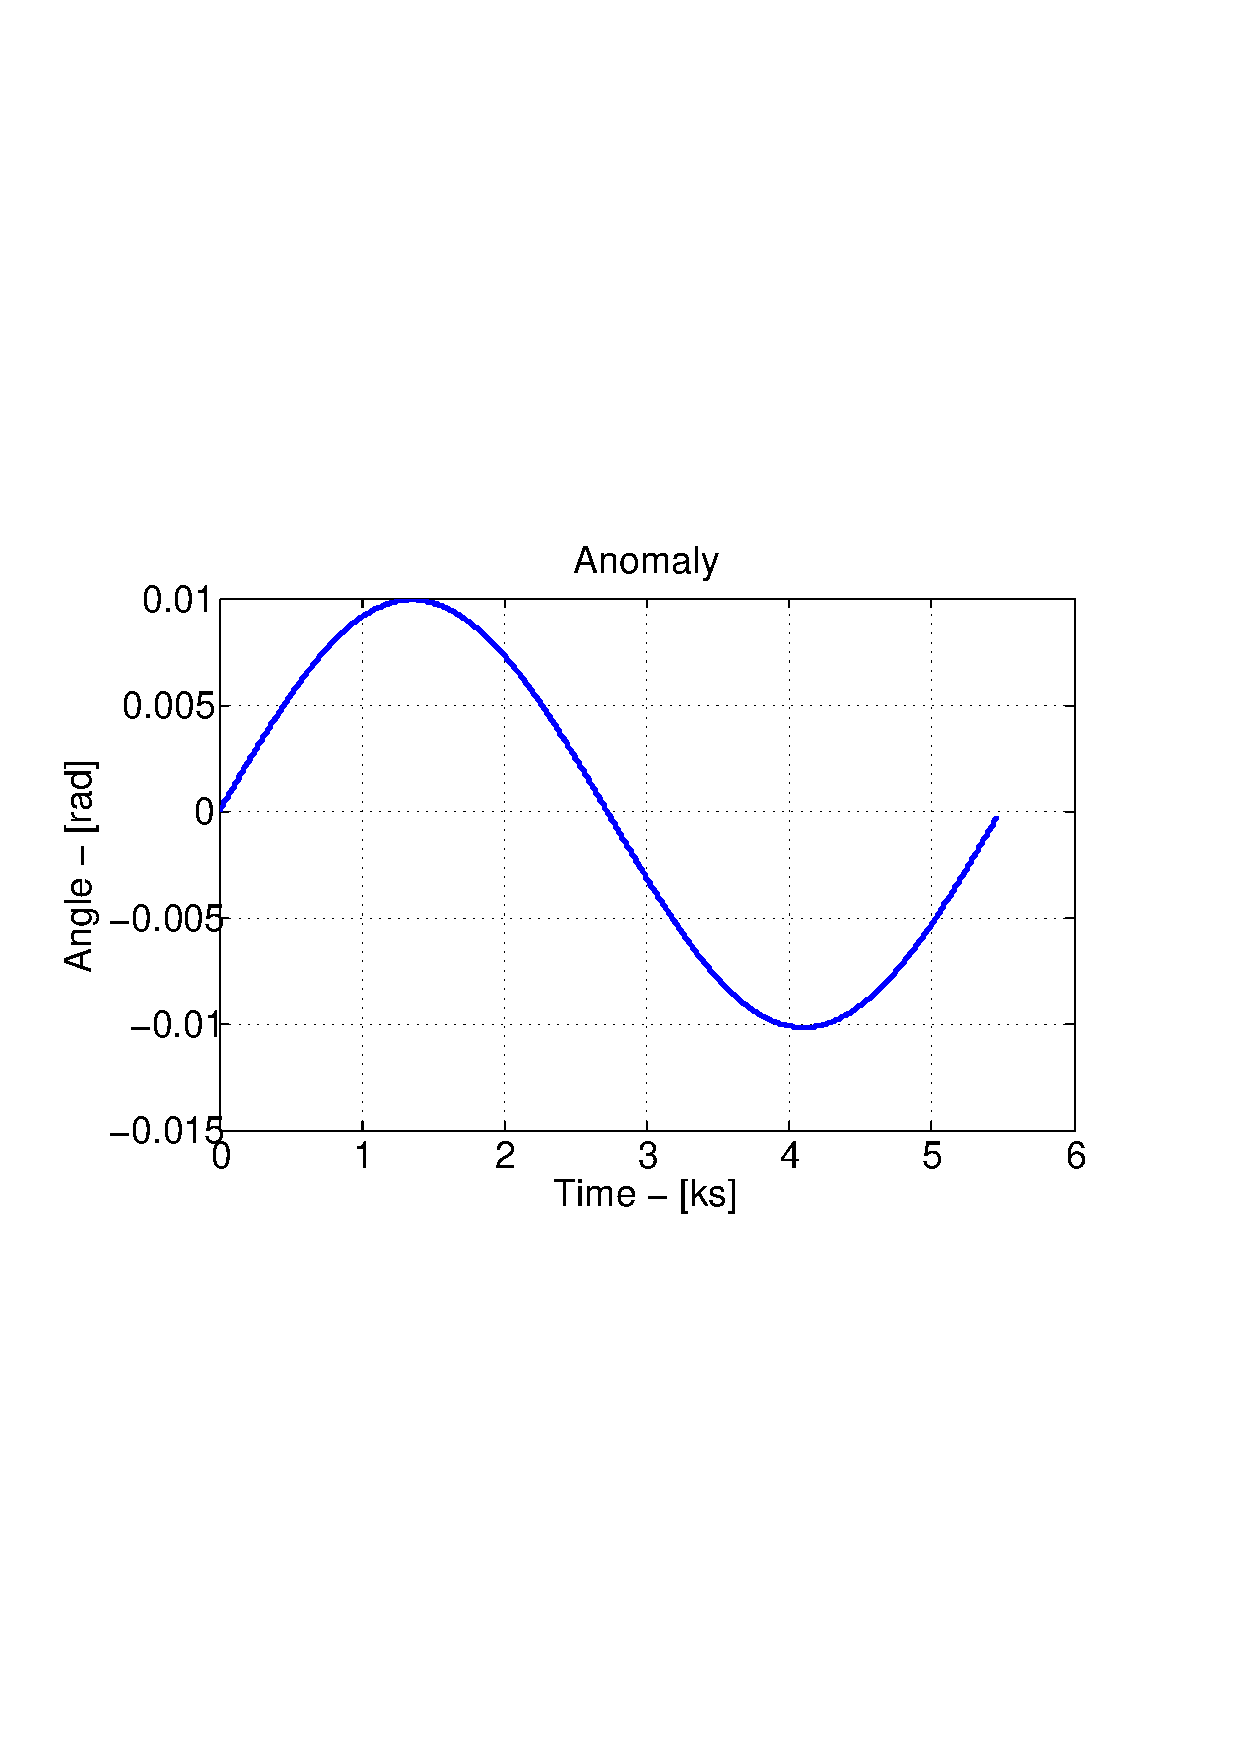
\includegraphics[width=.6\textwidth,clip=true,trim=1cm
	6cm
	1cm
	8cm]{modelling/orbit_dynamics/image/anomaly.pdf}
	\caption{\emph{Anomalia}--- differenza tra anomalia vera $\theta$ e velocità
	angolare media $\omega_0$}
\end{SCfigure}

\begin{SCfigure}[0.7][ht]
	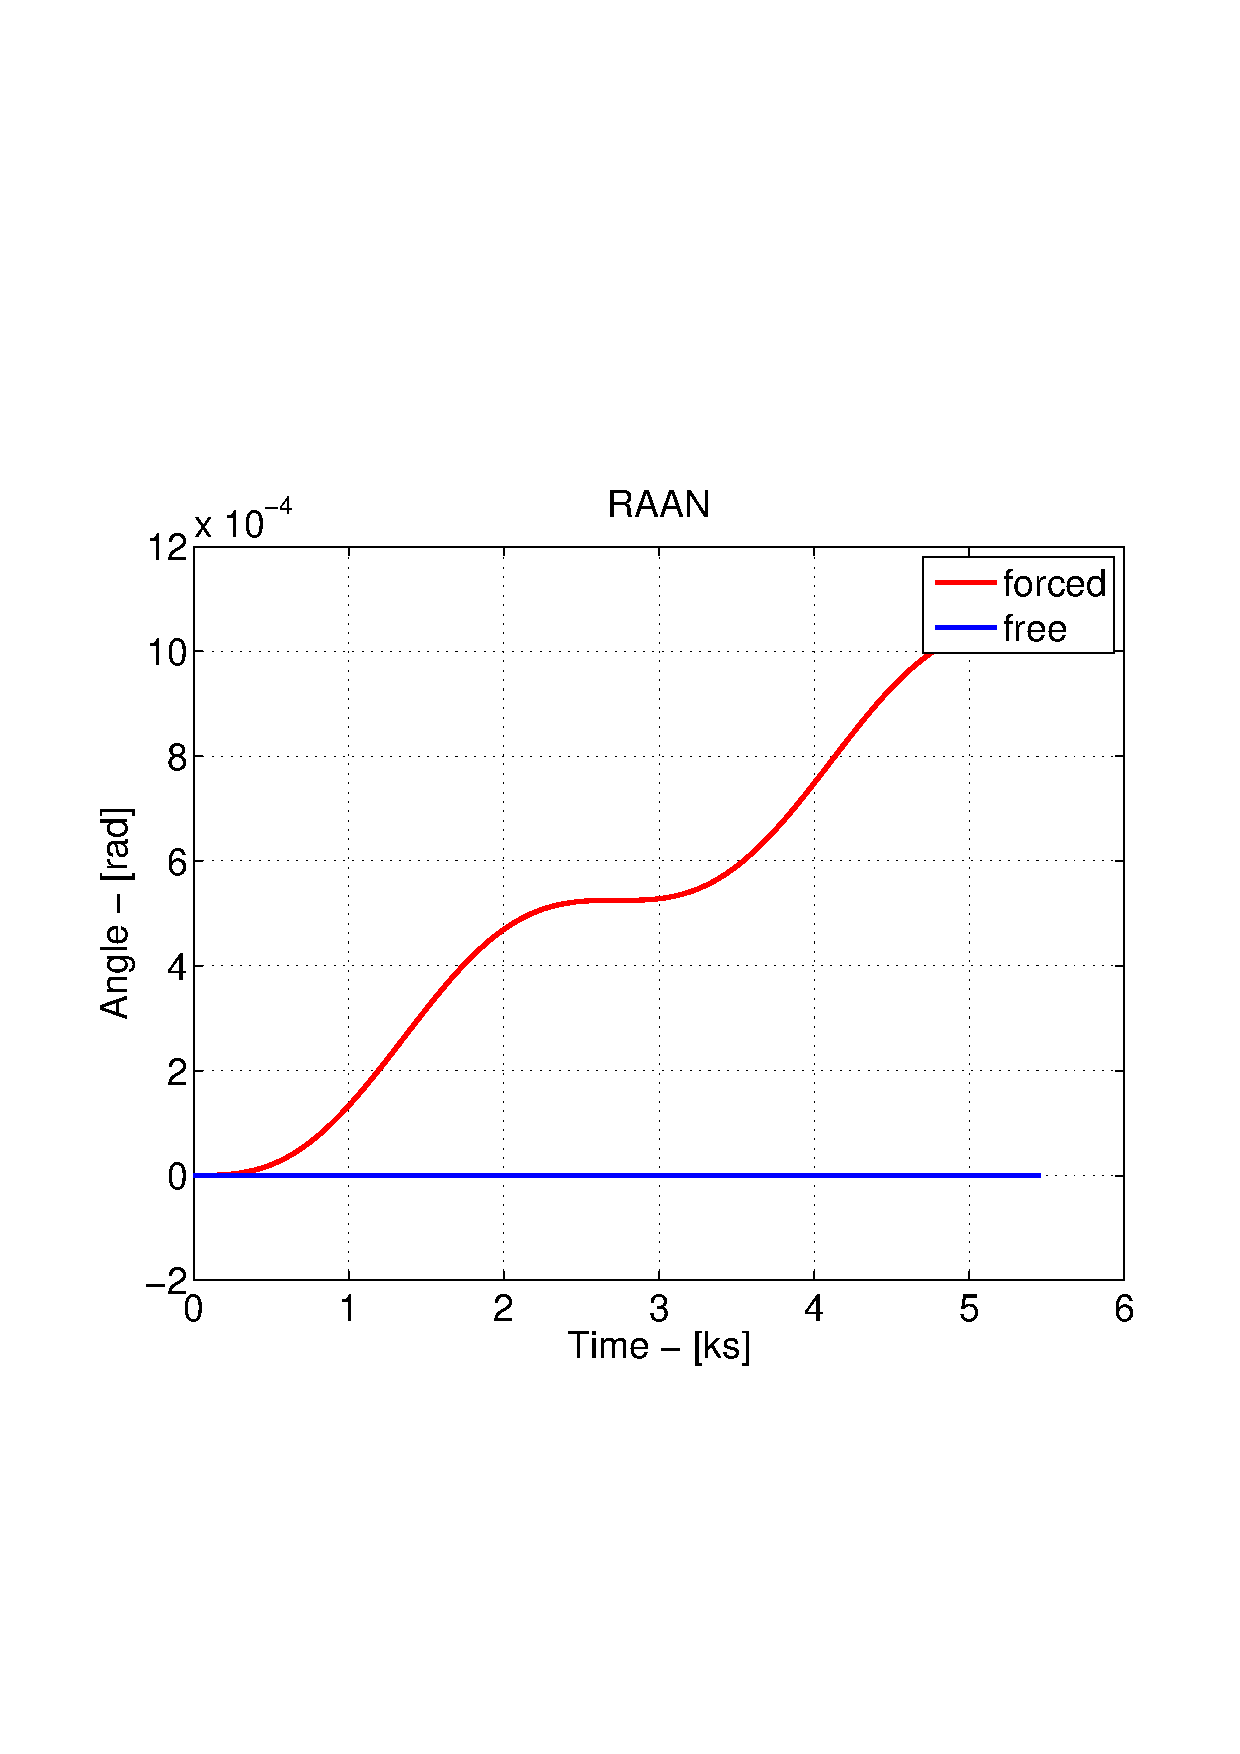
\includegraphics[width=.6\textwidth,clip=true,trim=1cm
	6cm
	1cm
	8cm]{modelling/orbit_dynamics/image/RAAN.pdf}
	\caption{\emph{RAAN}--- Right Ascension of the Ascending Node}
\end{SCfigure}